\subsection{Periodo di Progettazione di dettaglio e codifica}
\subsubsection{MPC01 - SPICE}
Ogni sigla presente in questa sezione fa riferimento a quanto descritto all'interno del documento \textit{NormeDiProgetto-v2.0.0} §A


\begin{table}[H]
    \rowcolors{2}{gray!25}{white}
    \rowcolors{2}{gray!25}{white}
        \renewcommand{\arraystretch}{1.5}
        \begin{tabular}{ m{0.15\textwidth}<{\centering}  m{0.055\textwidth}<{\centering} m{0.055\textwidth}<{\centering} m{0.055\textwidth}<{\centering} m{0.055\textwidth}<{\centering} m{0.055\textwidth}<{\centering} m{0.055\textwidth}<{\centering} m{0.055\textwidth}<{\centering} m{0.055\textwidth}<{\centering} m{0.055\textwidth}<{\centering} m{0.08\textwidth}<{\centering}}
	\rowcolor{darkblue}
	\textcolor{white}{\textbf{Processo}} &\textcolor{white}{\textbf{1.1}} &\textcolor{white}{\textbf{2.1}} &\textcolor{white}{\textbf{2.2}} &\textcolor{white}{\textbf{3.1}} &\textcolor{white}{\textbf{3.2}} &\textcolor{white}{\textbf{4.1}} &\textcolor{white}{\textbf{4.2}} &\textcolor{white}{\textbf{5.1}} &\textcolor{white}{\textbf{5.2}} &\textcolor{white}{\textbf{Livello}}\\ 


    Fornitura & F & F & F & P & L & N & N & N & N & 2 \\
    Sviluppo & F & F & F & F & F & N & N & N & N & 3 \\
    Documentazione & F & F & F & L & L & N & N & N & N & 2 \\
    Gestione della configurazione & F & F & F & N & N & N & N & N & N & 2 \\
    Gestione della qualità & F & F & F & F & F & N & N & N & N & 3 \\
    Verifica & F & F & F & L & P & N & N & N & N & 2 \\
   
    Gestione di processo & F & F & F & P & P & N & N & N & N & 2 \\
    Formazione dei membri del team & F & F & F & N & N & N & N & N & N & 2 \\
    
\end{tabular}       
\caption{Progettazione di dettaglio e codifica: MPC01 - SPICE}
\end{table}

\begin{figure}[H]
    \centering
    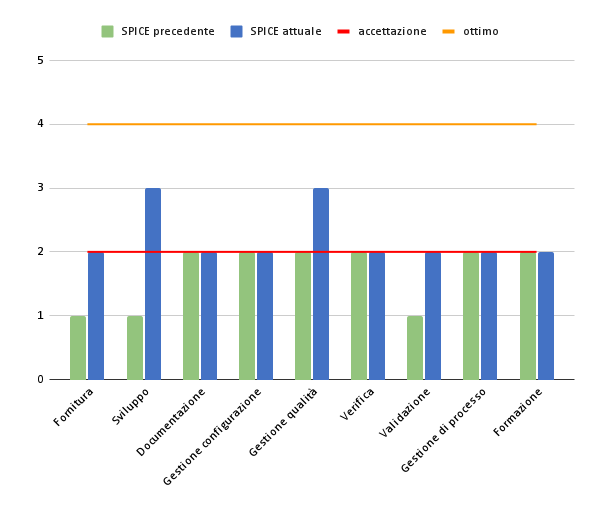
\includegraphics[scale=0.50]{Sezioni/images/pdc-spice.png}
    \caption{Progettazione di dettaglio e codifica: MPC01 - SPICE}
\end{figure}

   Alcune note sui risultati:
\begin{itemize}
\item Il processo di sviluppo passa dal livello 1 al livello 3
\item Il processo di gestione della qualità sale al livello 3
\item I processi di Fornitura e Validazione salgono al livello 2 raggiungendo così il valore tollerato
\item I restanti processi rimangono al livello 2, tuttavia buona parte di loro sono migliorati rispetto al periodo precedente ed è ragionevole pensare di raggiungere il livello 3 in futuro.
\end{itemize}


\subsubsection{MPC02 - BCWS}
\begin{figure}[H]
    \centering
    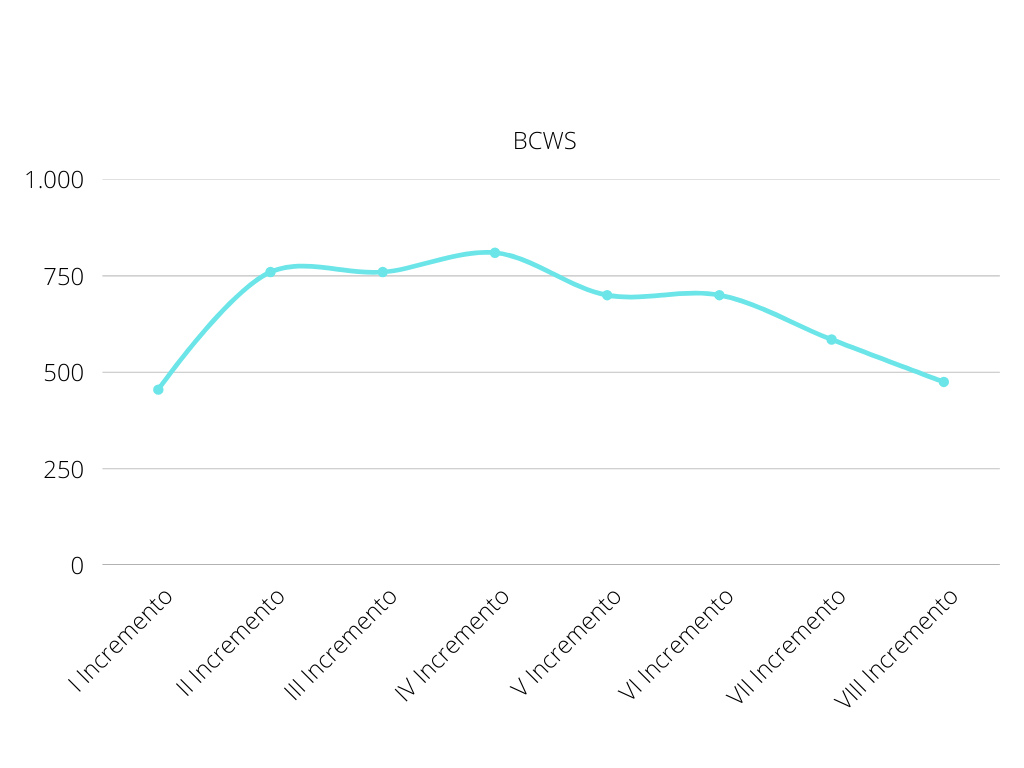
\includegraphics[scale=0.50]{Sezioni/images/pdc-BCWS.png}
    \caption{Progettazione di dettaglio e codifica: MPC02 - BCWS}
\end{figure}

\subsubsection{MPC03 - ACWP}
\begin{figure}[H]
    \centering
    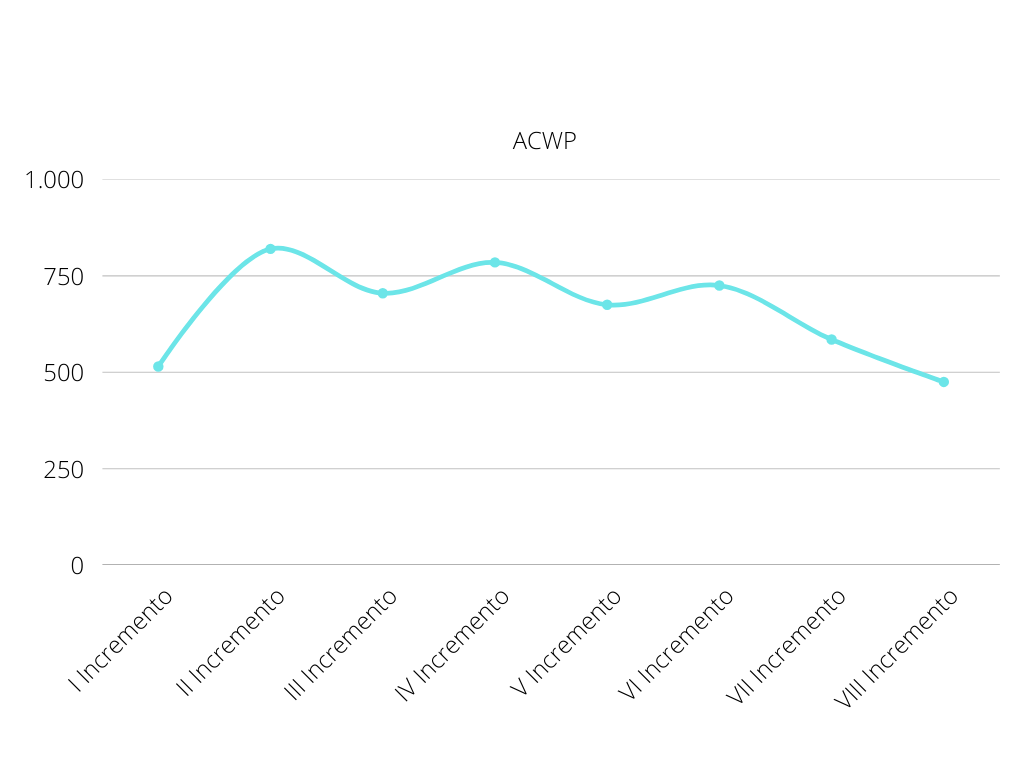
\includegraphics[scale=0.50]{Sezioni/images/pdc-ACWP.png}
    \caption{Progettazione di dettaglio e codifica: MPC03 - ACWP}
\end{figure}

\subsubsection{MPC04 - BCWP}
\begin{figure}[H]
    \centering
    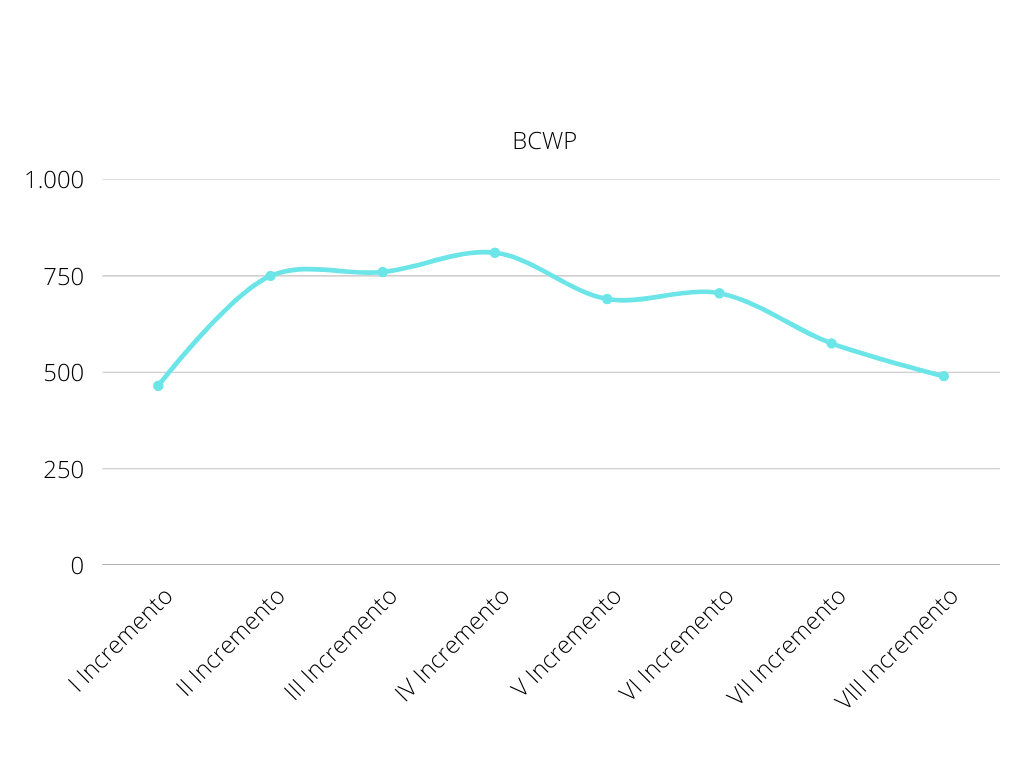
\includegraphics[scale=0.50]{Sezioni/images/pdc-BCWP.png}
    \caption{Progettazione di dettaglio e codifica: MPC04 - BCWP}
\end{figure}

\subsubsection{MPC05 - Schedule variance}
\begin{figure}[H]
    \centering
    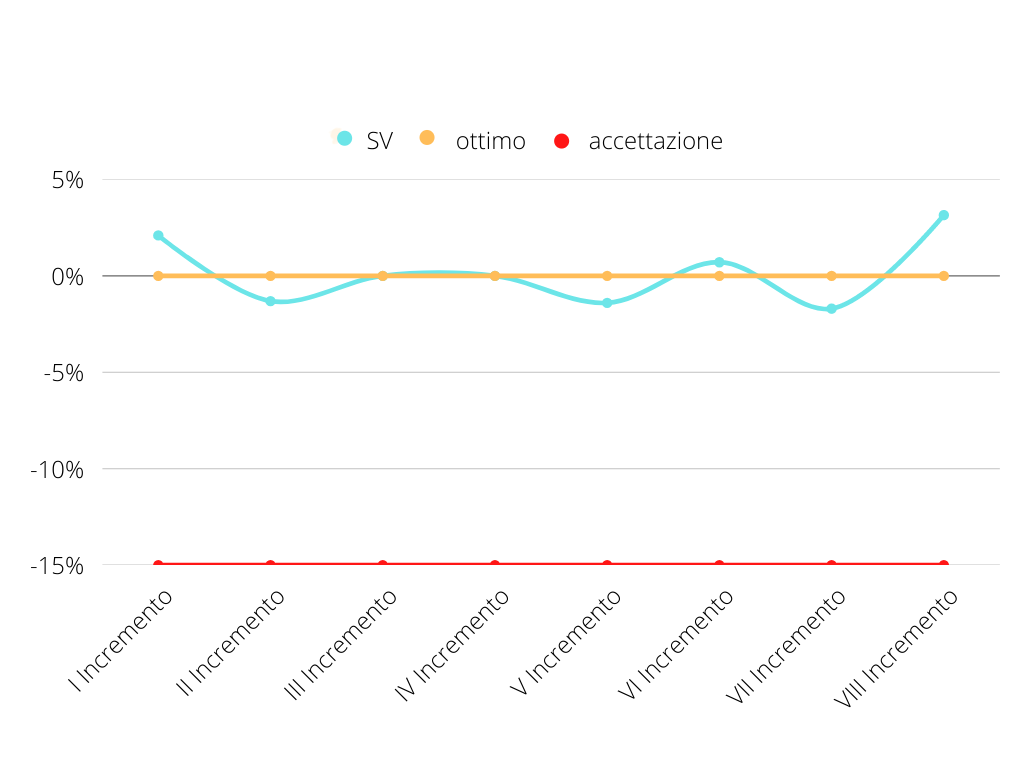
\includegraphics[scale=0.50]{Sezioni/images/pdc-SV.png}
    \caption{Progettazione di dettaglio e codifica: MPC05 - SV}
\end{figure}

\subsubsection{MPC06 - Budget variance}
\begin{figure}[H]
    \centering
    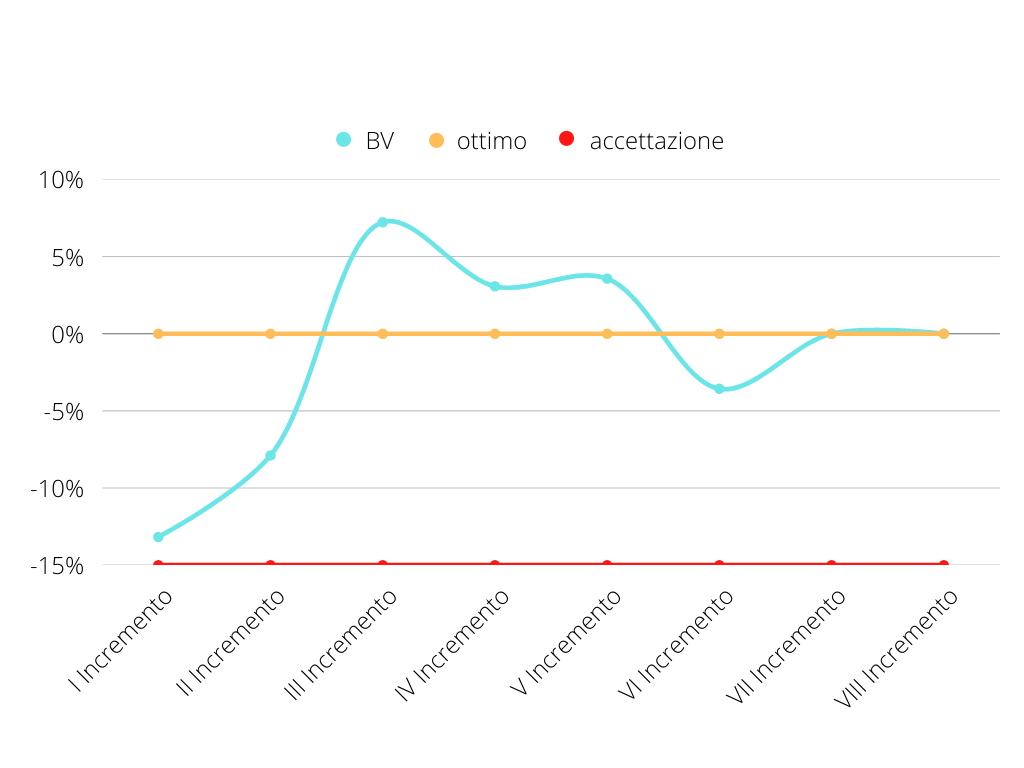
\includegraphics[scale=0.50]{Sezioni/images/pdc-BV.png}
    \caption{Progettazione di dettaglio e codifica: MPC06 - BV}
\end{figure}